\documentclass[11pt]{article}

\usepackage[margin=1in]{geometry}


\title{Chapter 3: Introduction to altitude-cognizant scalar Slepian functions}
\author{Kylee and  Sarah}

\usepackage{graphicx}
\graphicspath{ {./images/} }

%\userpackage{pdfpages}

\begin{document}
\maketitle


\subsubsection*{Introduction}

Now that we understand the classical scalar Slepian functions, we can consider the altitude of a satellite from which the data has been taken.   Atlitude-cognizant scalar Slepian functions can optimize the linear combination of spherical harmonics by a either a downward continuation from the satellite radius to the planet's surface or a upwardly continuation from the planet's surface to the satellite radius.  The altitude-cognizant scalar Slepian functions (AC-SSF) are constructed through the maximum spherical harmonic degree L, region of concentration, planet radius, and the average satellite radius.  Since there is 'negligible' potential field in the area between the planet's surface and the satellite altitude, we optimize the potential from the planet to create a model.  The AC-SSF optimizes the linear combination of scalar spherical harmonics to incorporate the satellite altitude at which the data was taken.  Basically, we are able to take the field data collected by a satellite at some altitude and, through an optimal linear combination, we are able to plot the field on the planet's surface. 
\\

\subsubsection*{Optimization}

To determine the optimal linear combination concentrated in the region, R, we must maximize the spacial ratio, $\lambda$.  
$$\lambda = \frac{\int_R(f_\uparrow(\hat{x}))^2dx}{\int_\Omega(f(\hat{x}))^2dx} = maximum$$

%$$f(\hat{x})= \sum_{L,m}^{L}{f_{L,m}Y_{L,m}(\hat{x})}$$

The following equation creates a linear combination with the spherical harmonic coefficients, $f_{L,m}$, and the spherical harmonic functions, $Y_{L,m}(\hat{x})$.  Because the AC-SSF includes the altitude component of the satellite, we denote our upward continuous linear combination as $f_\uparrow(\hat{x})$. 
 
$$f_\uparrow(\hat{x}) = \sum_{L,m}^{L}{(\frac{r_s}{r_p})^{-L-1}f_{L,m}Y_{L,m}(\hat{x})}$$

The main difference between the classical scalar Slepian functions and the AC-SSF is the factor including the satellite and planet radius.  

**For further explanation on the optimization of the linear combinations, see Plattner and Simons 2017 paper.**

\subsubsection*{MATLAB function and Plotting}

To acquire the Slepian functions, given a data set, we may use the function \verb+glmalphapotup+.  This function requires the following inputs: region, L, average radius to the satellite, and planet radius.  The outputs of this function are G, the matrix of spherical harmonic coefficients on the planet's surface, and $\vee$, the eigenvalues or the suitability factors. \\

However, to plot the Slepian function at satellite altitude, we must upward continue the functions by using: \verb+potup+.  This function requires the inputs: G, radius to the satellite, planet radius, Lmax, **? Lrange?...  The output will be the spherical harmonic coefficient vector for radial field at the new altitude. \\

To plot the Slepian function on the surface of the planet, we may use the same MATLAB functions as in the previous chapter, for the classical scalar Slepian functions: \verb+plotplm+ or \verb+plm2xyz+.  See the previous chapter for further explanation. \\

After initializing MATLAB or Octave, run \verb+demo_ch3+ to see the result below.

\begin{center}
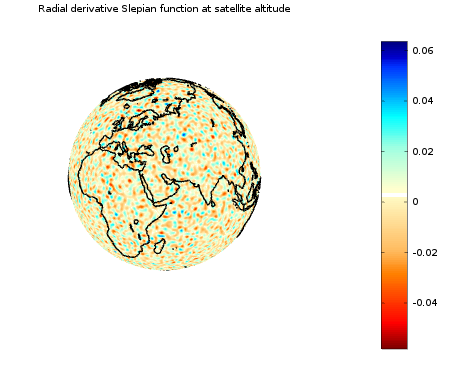
\includegraphics[scale=0.5]{ch3fig1.png}
\end{center}


\end{document}